\documentclass{beamer}

\usepackage[utf8]{inputenc}
\usepackage{hyperref}

\usetheme{Berkeley}
\beamertemplatenavigationsymbolsempty
\setbeamertemplate{headline}{}
 
\title{Geocoding in FoodChain-Lab}
\date{}
 
\begin{document}
\maketitle

\section{ }

\subsection{Aufgaben}
\begin{frame}
	\begin{itemize}
		\item Führen Sie ein Geocoding auf Basis folgenden Workflows durch: \url{https://github.com/SiLeBAT/BfROpenLabResources/raw/master/GitHubPages/workflows/Geocoding.zip}.
		\item Nutzen "Street", "HouseNumber", "City" und "Country" als Eingabeparameter für das Geocoding.
		\item Verwenden Sie den MapQuest Geocoding Service.
	\end{itemize}
\end{frame}
 
\subsection{1}
\begin{frame}
	\begin{center}
  		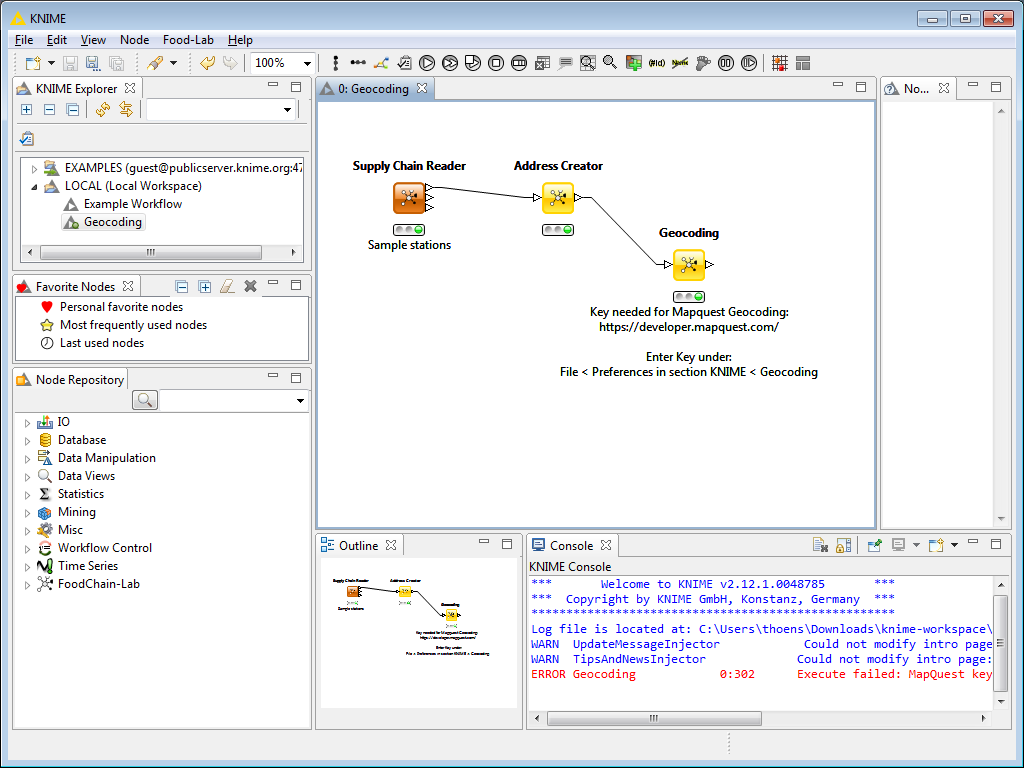
\includegraphics[height=0.6\textheight]{1.png}
	\end{center}
	\begin{itemize}
		\item Importieren Sie den Geocoding Workflow von \url{https://github.com/SiLeBAT/BfROpenLabResources/raw/master/GitHubPages/workflows/Geocoding.zip}.
		\item In diesem Tutorial benutzen wir den MapQuest Geocoding Service.
	\end{itemize}
\end{frame}

\subsection{2}
\begin{frame}
	\begin{center}
  		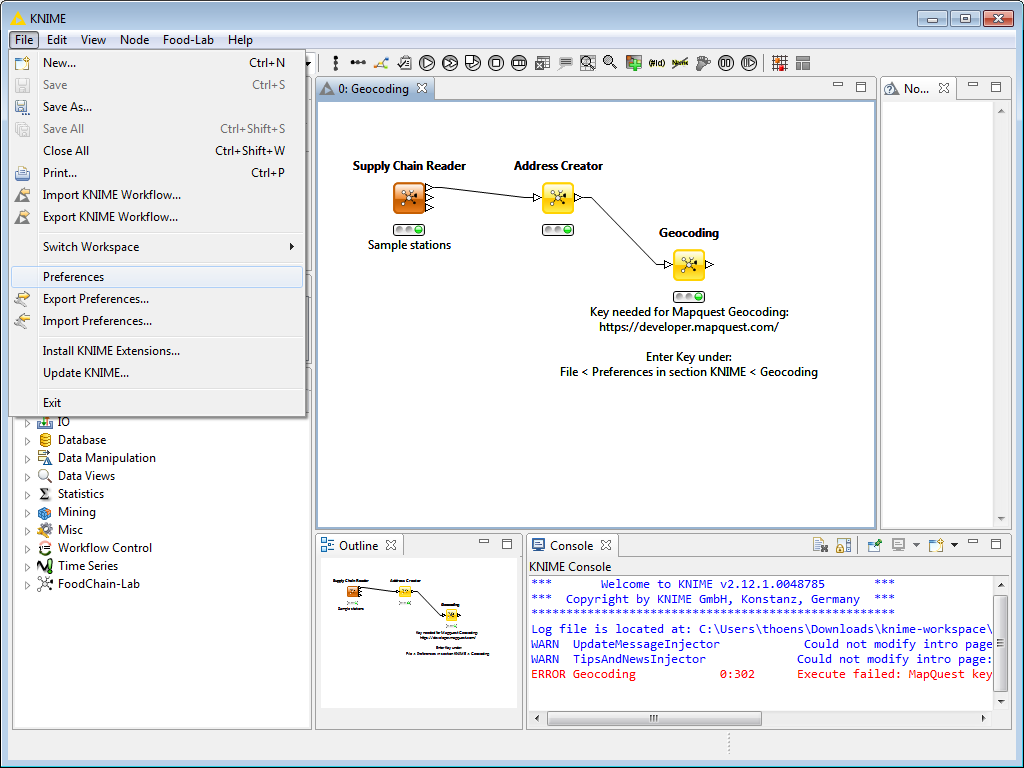
\includegraphics[height=0.6\textheight]{2.png}
	\end{center}
	\begin{itemize}		
		\item Für MapQuest müssen Sie sich registrieren und einen App-Key erstellen unter: \url{https://developer.mapquest.com}
		\item Dieser App-Key muss in den KNIME-Einstellungen eingegeben werden.
		\item Wählen Sie \textbf{File $<$ Preferences} in der Menüleiste.
	\end{itemize}
\end{frame}

\subsection{3}
\begin{frame}
	\begin{center}
  		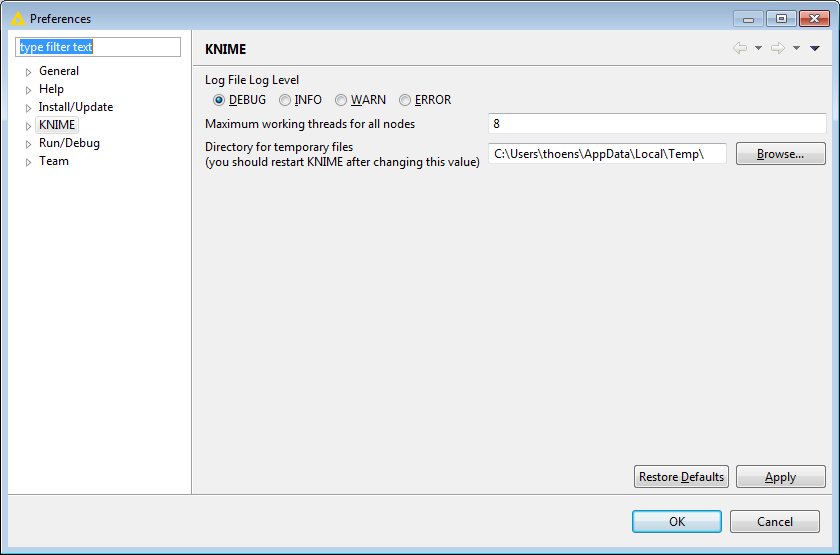
\includegraphics[height=0.6\textheight]{3.png}
	\end{center}
	\begin{itemize}
		\item Nun erscheint der Einstellungs-Dialog.
		\item Hier können Sie alle Einstellungen für KNIME und FoodChain-Lab vornehmen.
	\end{itemize}
\end{frame}

\subsection{4}
\begin{frame}
	\begin{center}
  		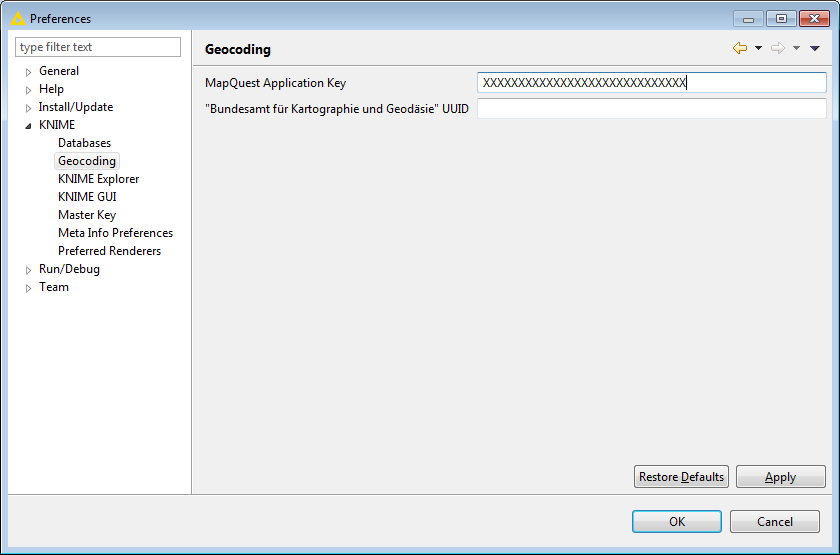
\includegraphics[height=0.6\textheight]{4.png}
	\end{center}
	\begin{itemize}
		\item Wählen Sie \textbf{KNIME $<$ Geocoding} im Navigations-Baum auf der linken Seite.
		\item Geben Sie ihren \textbf{MapQuest Application Key} ein und klicken Sie \textbf{OK}.
	\end{itemize}
\end{frame}

\subsection{5}
\begin{frame}
	\begin{center}
  		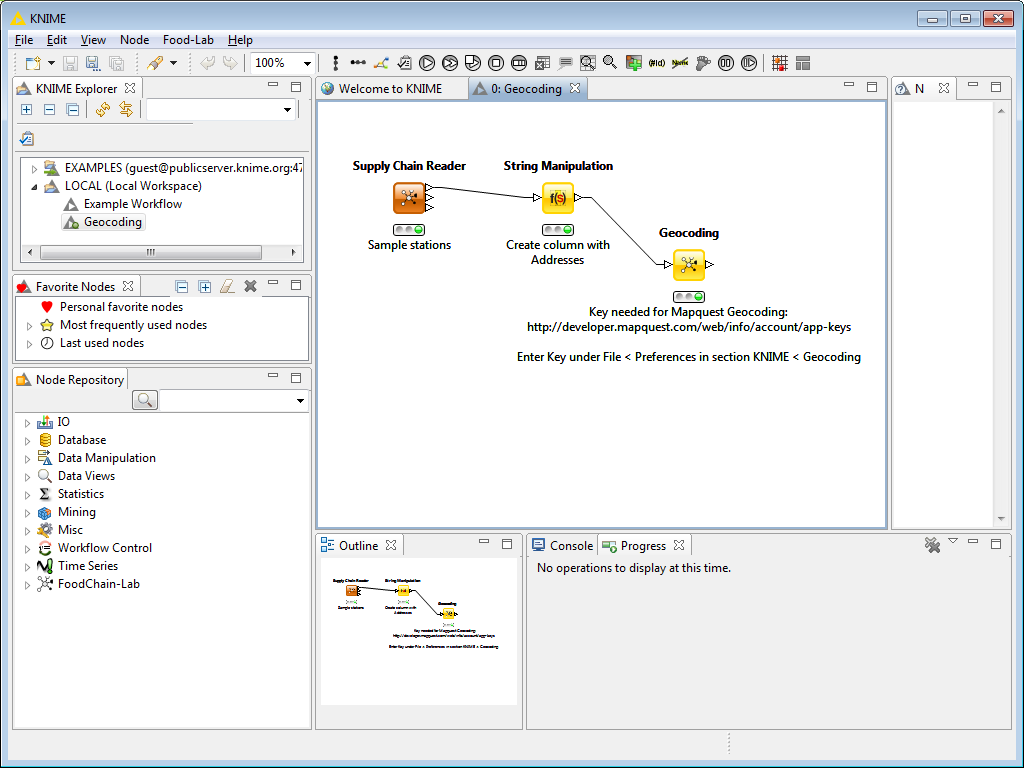
\includegraphics[height=0.5\textheight]{5.png}
	\end{center}
	\begin{itemize}
		\item Um das Geocoding auszuführen benötigen wir eine Spalte mit Adressen. Der \textbf{Supply Chain Reader} gibt allerdings alle Teile der Adresse (Straße, Stadt, ...) in verschiedenen Spalten aus.
		\item Die Adress-Spalte wir mit dem \textbf{Address Creator}-Knoten erstellt.
		\item Machen Sie einen Doppelklick auf diesen Knoten um den Konfigurationsdialog zu öffnen.
	\end{itemize}
\end{frame}

\subsection{6}
\begin{frame}
	\begin{center}
  		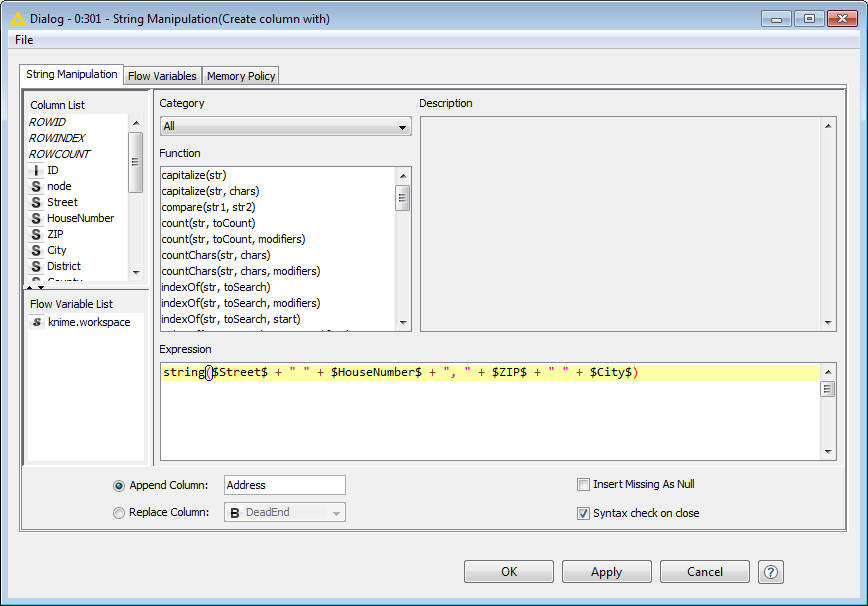
\includegraphics[height=0.6\textheight]{6.png}
	\end{center}
	\begin{itemize}
		\item In diesem Dialog können Sie definieren welche Spalten für die Adress-Spalte benutzt werden sollen.		
	\end{itemize}
\end{frame}

\subsection{7}
\begin{frame}
	\begin{center}
  		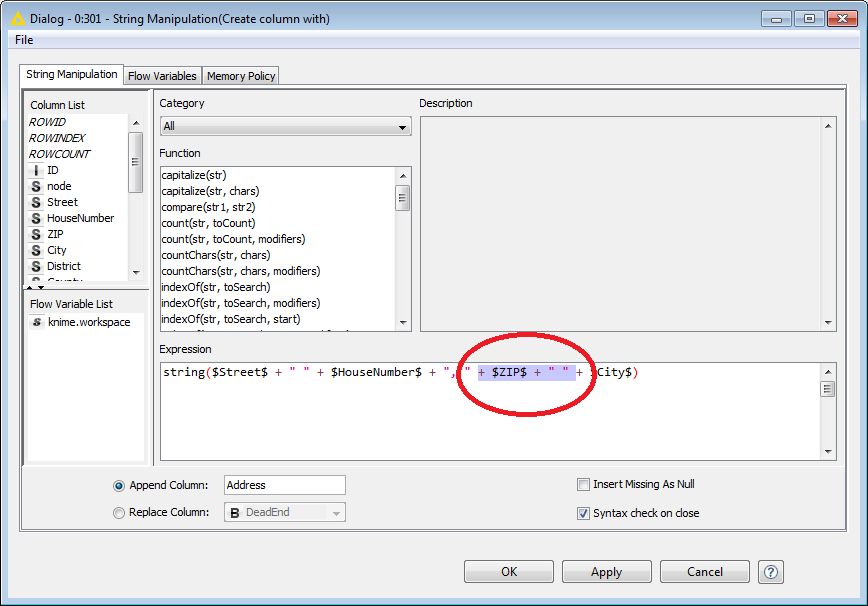
\includegraphics[height=0.5\textheight]{7.png}
	\end{center}
	\begin{itemize}
		\item Da wir das Geocoding basierend auf "Street", "HouseNumber", "City" and "Country" durchführen wollen, müssen wir \textbf{Country Column} auf "Country" setzen und \textbf{Postal Code Column} auf "none"
		\item Klicken Sie \textbf{OK} um den Dialog zu schließen.
	\end{itemize}
\end{frame}

\subsection{8}
\begin{frame}
	\begin{center}
  		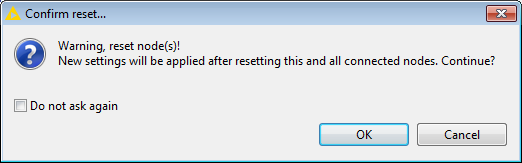
\includegraphics[width=0.9\textwidth]{8.png}
	\end{center}
	\begin{itemize}
		\item Da wir die Einstellungen geändert haben, muss der Knoten resettet werden. 
		\item Klicken Sie \textbf{OK}.
	\end{itemize}
\end{frame}

\subsection{9}
\begin{frame}
	\begin{center}
  		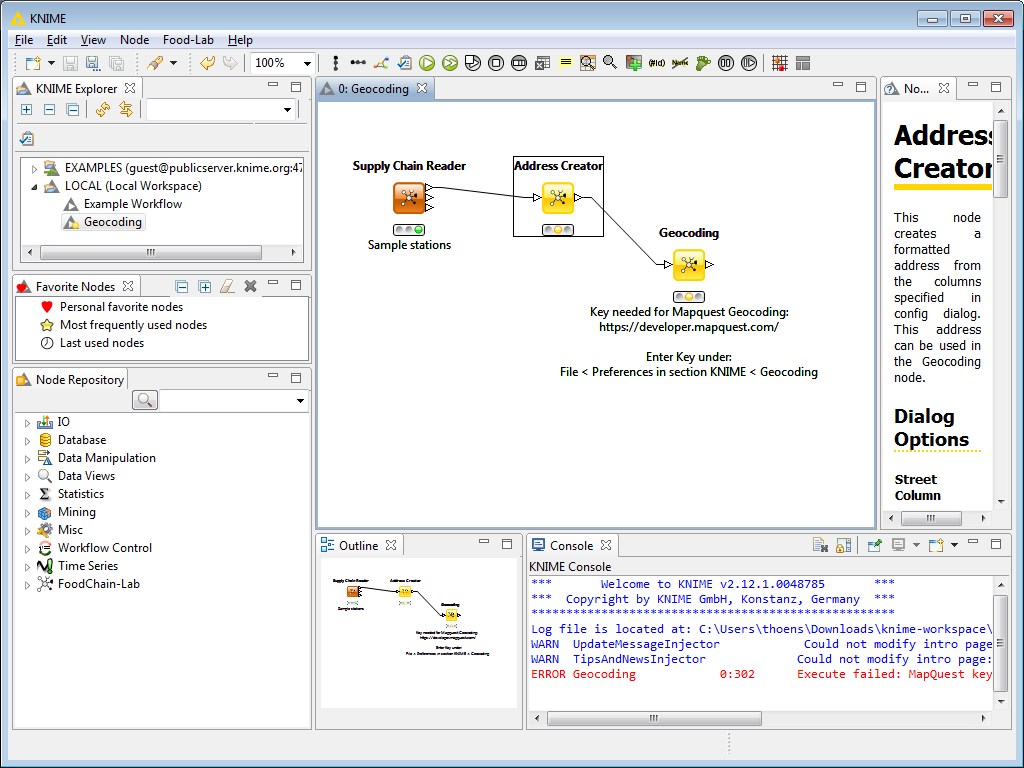
\includegraphics[height=0.6\textheight]{9.png}
	\end{center}
	\begin{itemize}
		\item Wir haben den \textbf{Address Creator} nun passend konfiguriert und ihn neu ausführen.
	\end{itemize}
\end{frame}

\subsection{10}
\begin{frame}
	\begin{center}
  		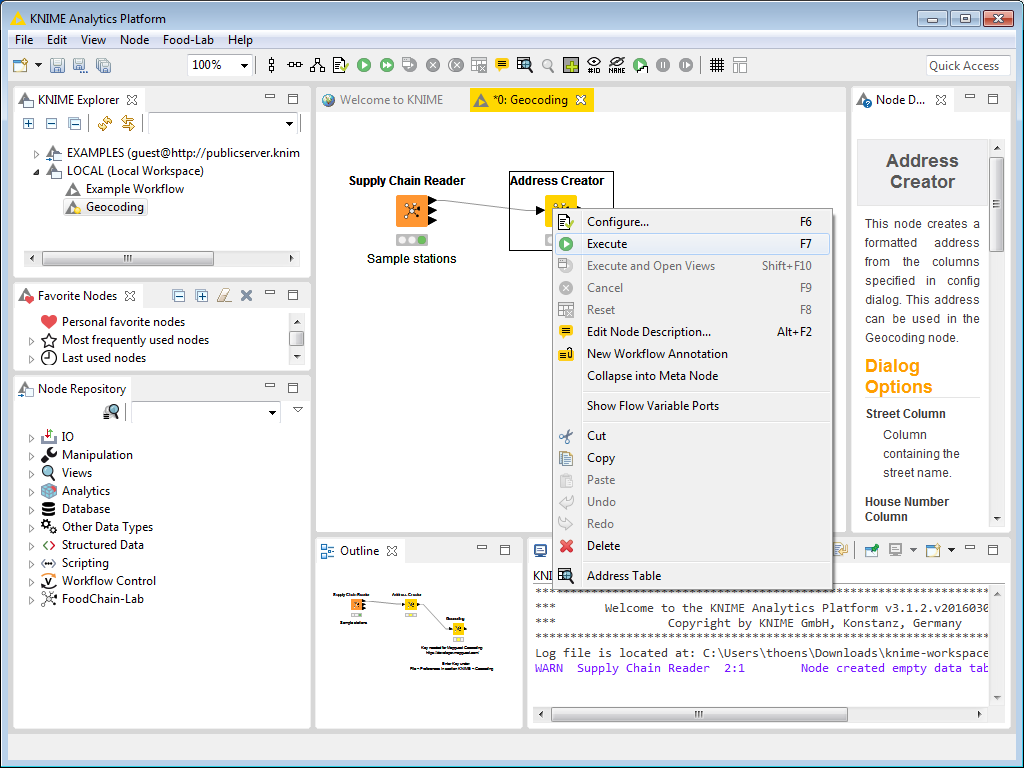
\includegraphics[height=0.6\textheight]{10.png}
	\end{center}
	\begin{itemize}
		\item Machen Sie einen Rechtsklick auf den \textbf{Address Creator} und wählen Sie \textbf{Execute}.
	\end{itemize}
\end{frame}

\subsection{11}
\begin{frame}
	\begin{center}
  		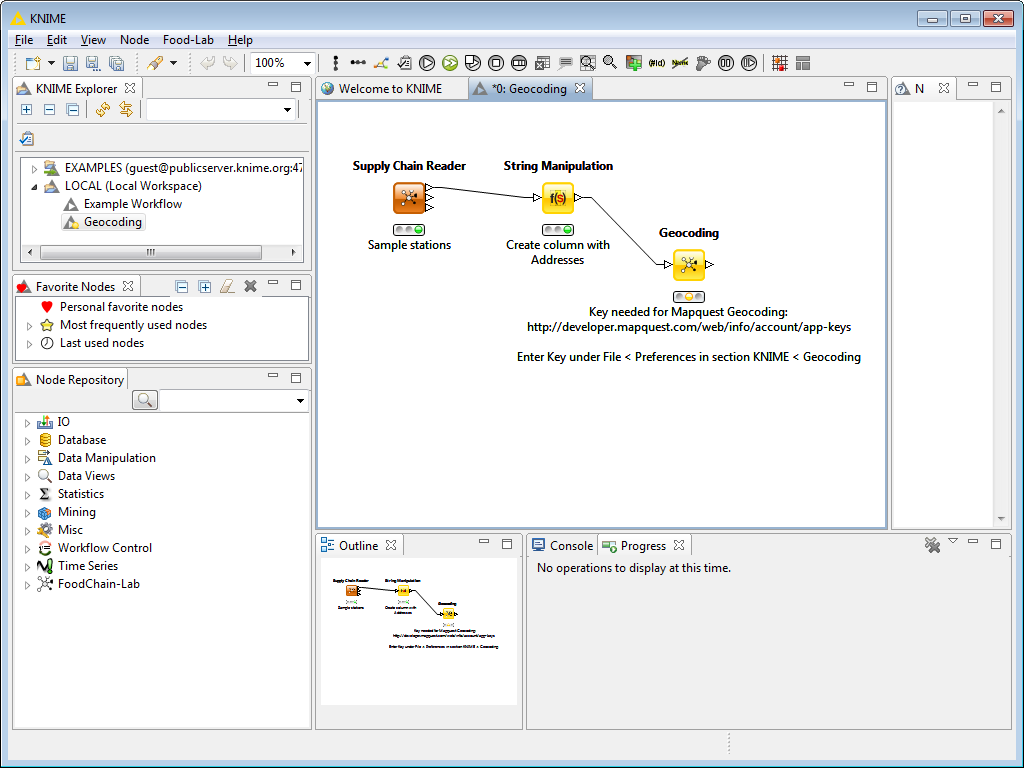
\includegraphics[height=0.6\textheight]{11.png}
	\end{center}
	\begin{itemize}
		\item Nun können wir das Geocoding konfigurieren.
		\item Machen Sie einen Doppelklick auf den \textbf{Geocoding}-Knoten um den Dialog zu öffnen.
	\end{itemize}
\end{frame}

\subsection{12}
\begin{frame}
	\begin{center}
  		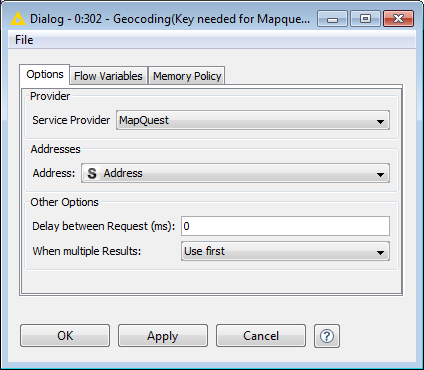
\includegraphics[height=0.6\textheight]{12.png}
	\end{center}
	\begin{itemize}
		\item Hier können Sie welchen \textbf{Service Provider} Sie nutzen möchten und welche Spalte die Adressen enthält.
		\item Beide Einstellungen sind bereits korrekt, also brauchen wir hier nichts ändern.
	\end{itemize}
\end{frame}

\subsection{13}
\begin{frame}
	\begin{center}
  		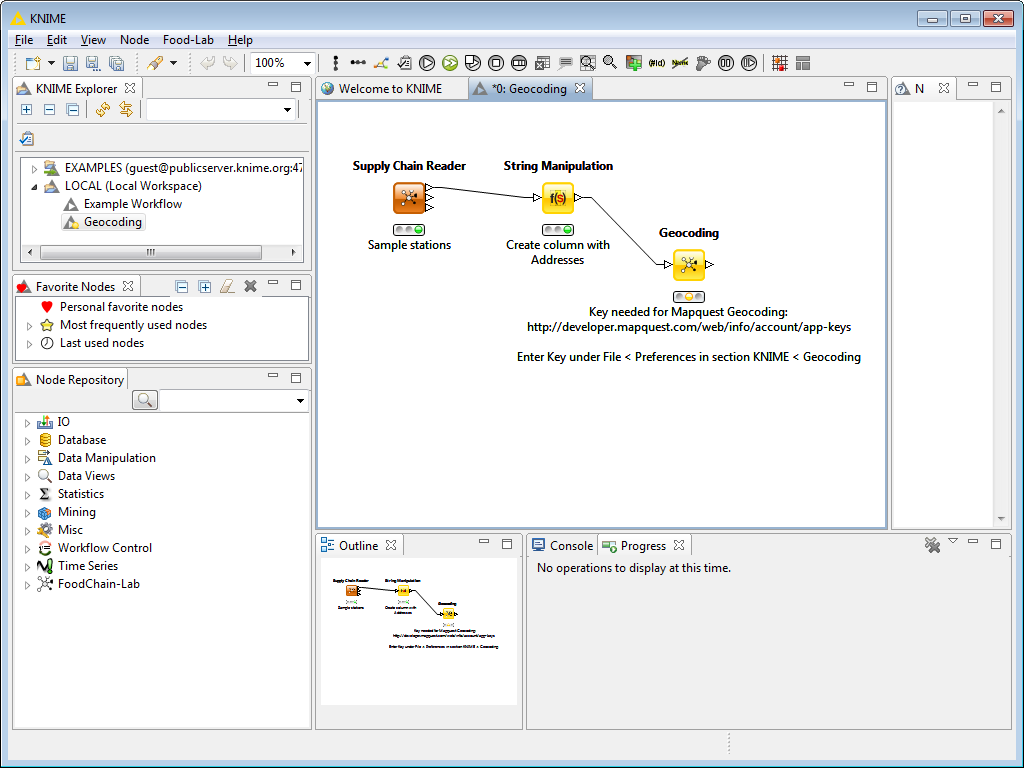
\includegraphics[height=0.4\textheight]{13.png}
	\end{center}
	\begin{itemize}
		\item Es passiert häufig, dass der Geocoding Service zu einer Anfrage mehrere Resultate liefert (z.B. wenn es mehrere Straßen mit demselben Name in einer Stadt gibt).
		\item Wir müssen definieren was in diesem Fall passieren soll: kein Resultat nehmen, das erste Resultat nehmen oder das passende Resultat manuell auswählen.
		\item Manuelles Auswählen ist bei großen Datenmengen sehr arbeitsaufwendig, deshalb wählen wir hier einfach \textbf{Use first} und klicken \textbf{OK}.
	\end{itemize}
\end{frame}

\subsection{14}
\begin{frame}
	\begin{center}
  		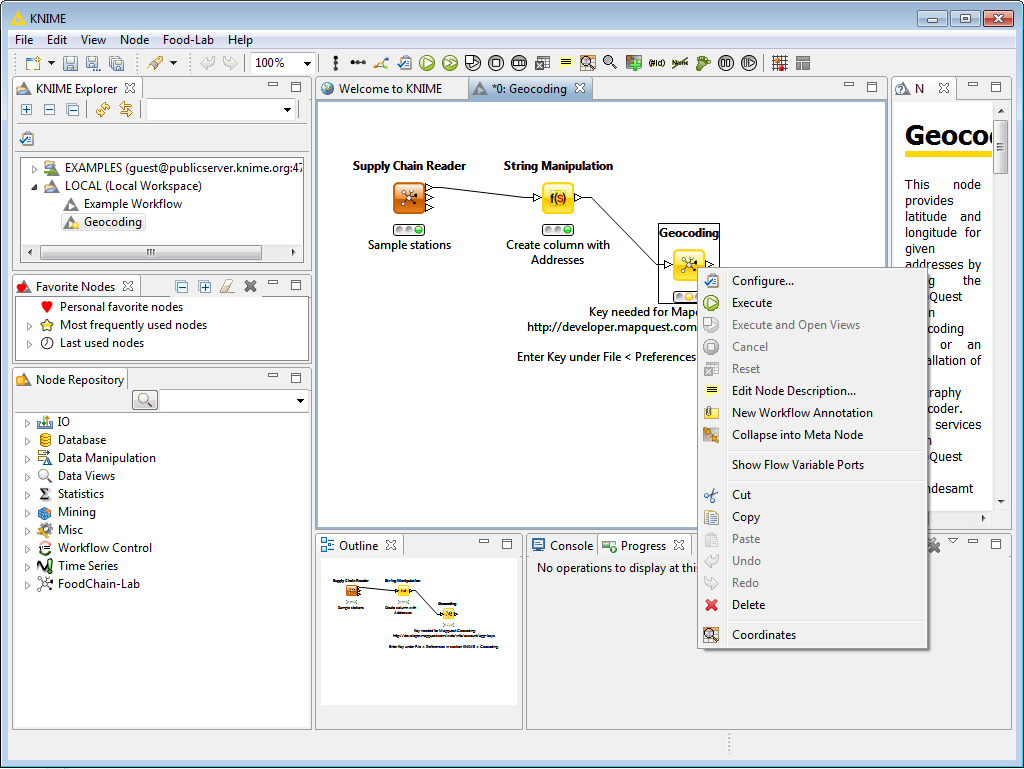
\includegraphics[height=0.6\textheight]{14.png}
	\end{center}
	\begin{itemize}
		\item Machen Sie einen Rechtsklick auf den \textbf{Geocoding}-Knoten und wählen Sie \textbf{Execute}.
	\end{itemize}
\end{frame}

\subsection{15}
\begin{frame}
	\begin{center}
  		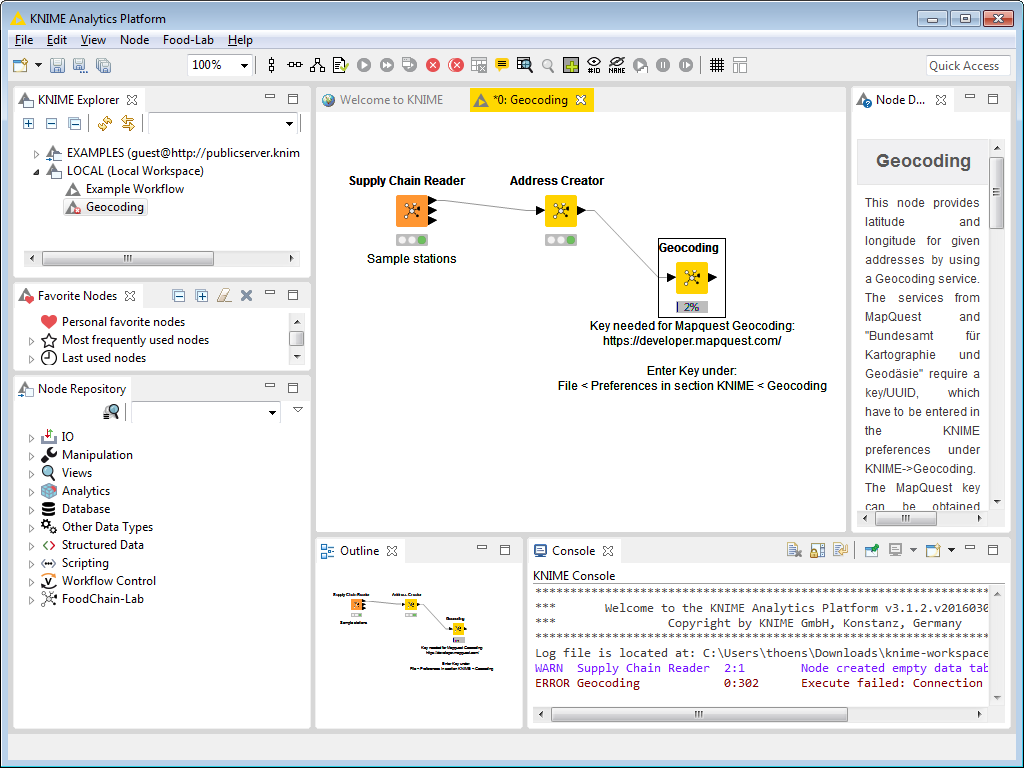
\includegraphics[height=0.6\textheight]{15.png}
	\end{center}
	\begin{itemize}
		\item Die Ausführung kann eine Weile dauern.
		\item Unter dem Knoten wird angezeigt welcher Prozentsatz der Daten bereits bearbeitet wurde.
	\end{itemize}
\end{frame}

\subsection{16}
\begin{frame}
	\begin{center}
  		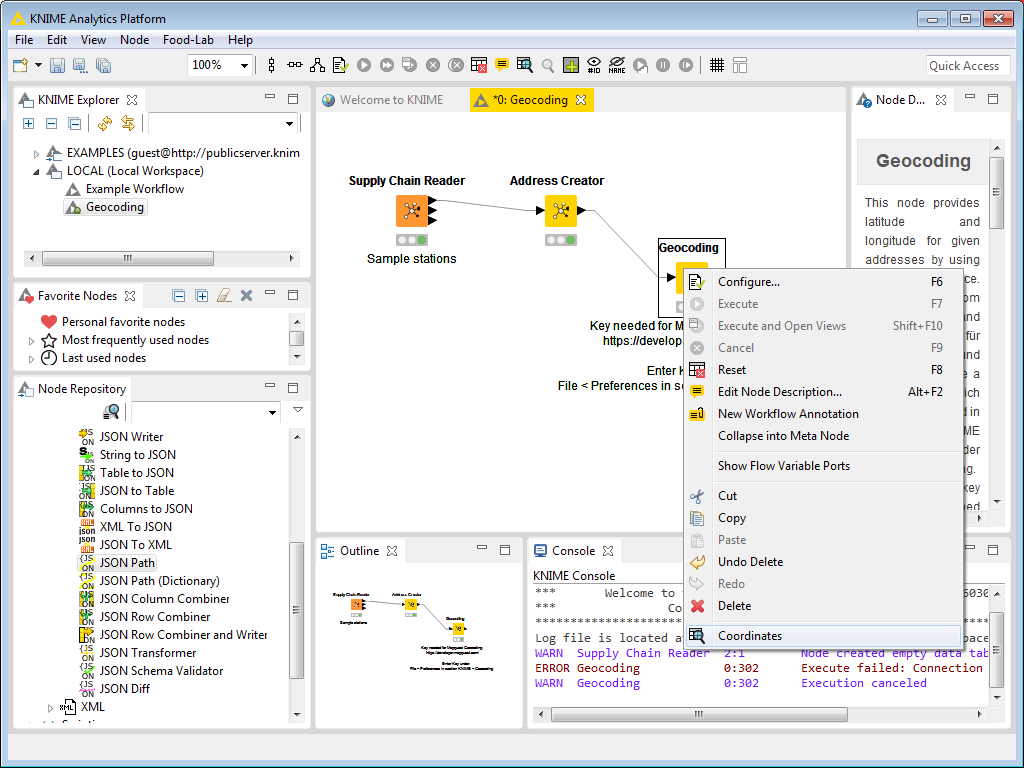
\includegraphics[height=0.6\textheight]{16.png}
	\end{center}
	\begin{itemize}
		\item Wenn die Ausführung beendet ist, können wir uns die Resultate anschauen.
		\item Machen Sie einen Rechtsklick auf den \textbf{Geocoding}-Knoten und wählen Sie \textbf{Coordinates}.
	\end{itemize}
\end{frame}

\subsection{17}
\begin{frame}
	\begin{center}
  		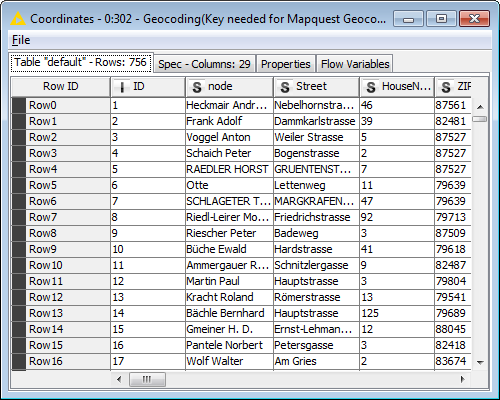
\includegraphics[height=0.6\textheight]{17.png}
	\end{center}
	\begin{itemize}
		\item In dem Dialog können Sie sich die gesamte Datentabelle anschauen.
	\end{itemize}
\end{frame}

\subsection{18}
\begin{frame}
	\begin{center}
  		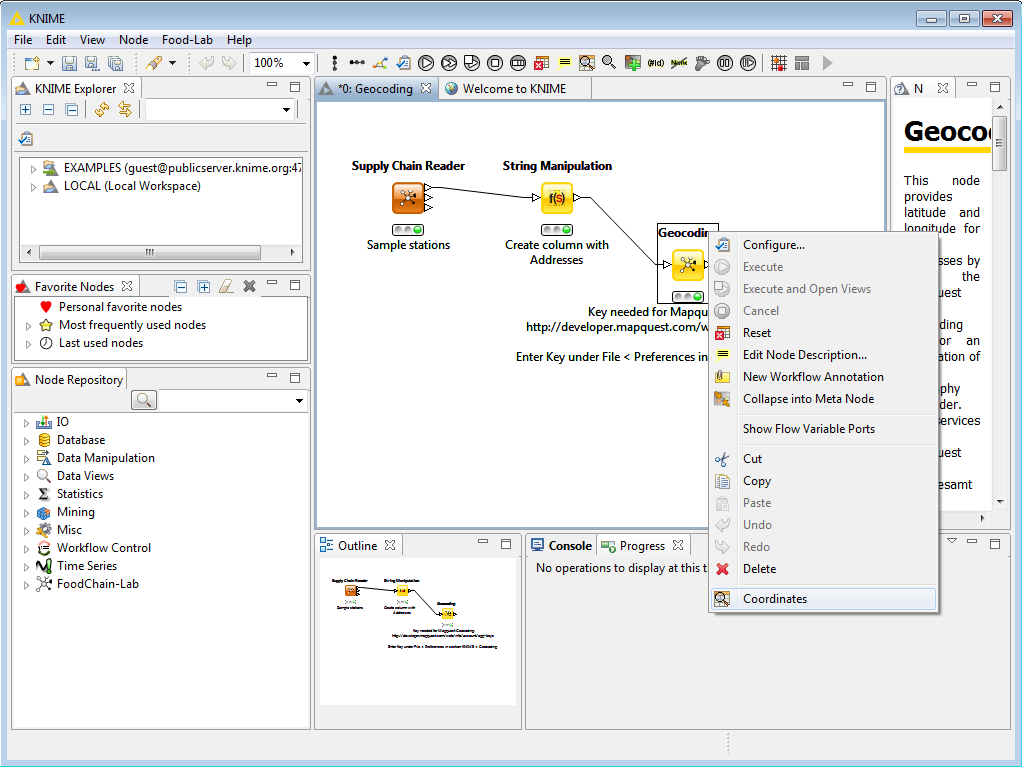
\includegraphics[height=0.6\textheight]{18.png}
	\end{center}
	\begin{itemize}
		\item Scrollen Sie ganz nach rechts um sich die Spalten mit geographischer Breite und Länge anzuschauen (die zwei Spalten ganz rechts).
		\item Bei mehrere Geocoding Anfragen haben wir falsche Ergebnisse. MapQuest hat Koordinaten für die USA geliefert, obwohl alle Addressen aus Deutschland sind.
	\end{itemize}
\end{frame}

\end{document}